\documentclass{article}

\usepackage{graphicx}
\usepackage{tikz}
\usepackage{tikzsymbols}
\usetikzlibrary{calc,patterns,shapes.geometric}
\pagestyle{empty}
\usepackage[margin=0pt]{geometry}
\geometry{papersize={14in,12in}}

\def\centerarc[#1](#2)(#3:#4:#5){\draw[#1] ($(#2)+({#5*cos(#3)},{#5*sin(#3)})$) arc (#3:#4:#5);}

\begin{document}
	\begin{figure}
		\centering
		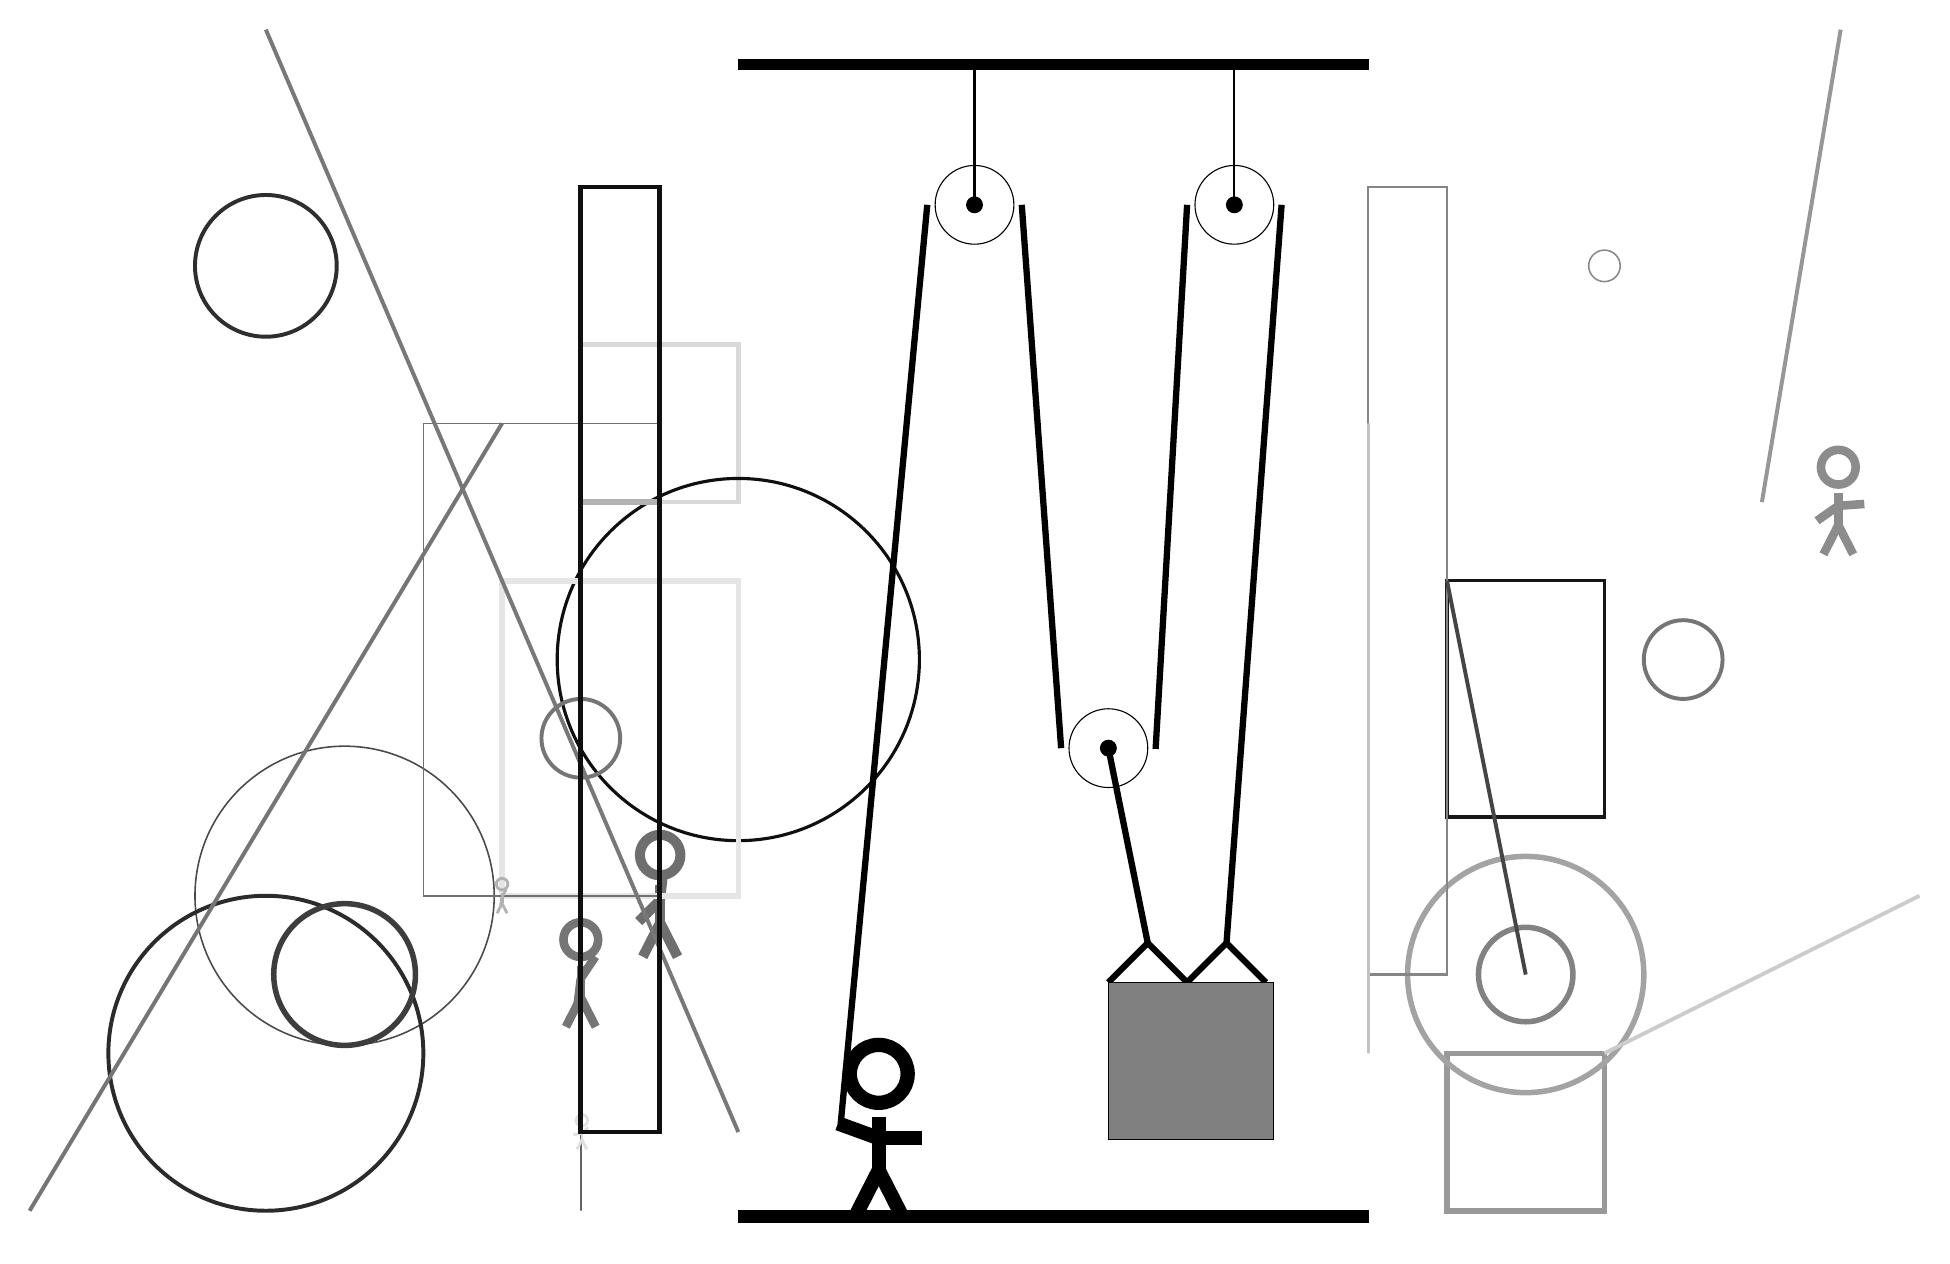
\begin{tikzpicture}
			%%%%% START %%%%%
			
			\draw[fill=black] (-2, 11.5) rectangle (6, 11.625);
			
			\draw (1, 9.775) circle (0.5);
			\draw[fill=black] (1, 9.775) circle (0.1);
			\draw[thick] (1, 9.775) -- (1, 11.5);
			
			\draw (4.3, 9.775) circle (0.5);
			\draw[fill=black] (4.3, 9.775) circle (0.1);
			\draw[thick] (4.3, 9.775) -- (4.3, 11.5);
			
			\draw (2.7, 2.875) circle (0.5);
			\draw[fill=black] (2.7, 2.875) circle (0.1);
			
			\draw [line width=0.5mm, color=black!54](10, 4) circle (0.5);
			
			\draw[line width=0.2mm, color=black!61] (-4, 5) rectangle (-4, -3);
			\node[line width=0.4mm, color=black!12] at (-4, -2) {\Strichmaxerl[2][9][43]};
			\draw[line width=0.4mm, color=black!91] (7, 5) rectangle (9, 2);
			\draw[line width=0.7mm, color=black!40] (7, -3) rectangle (9, -1);
			
			\draw[line width=0.6mm, color=black!15] (-2, 8) rectangle (-4, 6);
			
			\node[line width=0.3mm, color=black!45] at (12, 6) {\Strichmaxerl[6][35][4]};
			\draw [line width=0.4mm, color=black!94](-2, 4) circle (2.3);
			\draw [line width=0.7mm, color=black!36](8, 0) circle (1.5);
			\draw[line width=0.5mm, color=black!41](11, 6) -- (12, 12);
			\node[line width=0.6mm, color=black!57] at (-3, 1) {\Strichmaxerl[7][45][84]};
			
			\draw [line width=0.7mm, color=black!49](8, 0) circle (0.6);
			\draw[line width=0.5mm, color=black!20](9, -1) -- (13, 1);
			
			\draw[line width=0.3mm, color=black!48] (6, 10) rectangle (7, 0);
			\draw [line width=0.5mm, color=black!54](-4, 3) circle (0.5);
			\draw [line width=0.2mm, color=black!71](-7, 1) circle (1.9);
			
			\draw [line width=0.5mm, color=black!83](-8, -1) circle (2.0);
			\draw [line width=0.7mm, color=black!76](-7, 0) circle (0.9);
			\draw[line width=0.5mm, color=black!73](8, 0) -- (7, 5);
			
			\draw[line width=0.4mm, color=black!24] (6, 7) rectangle (6, -1);
			\draw[line width=0.7mm, color=black!10] (-2, 5) rectangle (-5, 1);
			\draw[line width=0.2mm, color=black!56] (-3, 7) rectangle (-6, 1);
			\draw [line width=0.5mm, color=black!82](-8, 9) circle (0.9);
			\draw[line width=0.7mm, color=black!30] (-3, 6) rectangle (-4, 6);
			\draw[line width=0.5mm, color=black!53](-2, -2) -- (-8, 12);
			\node[line width=0.7mm, color=black!30] at (-5, 1) {\Strichmaxerl[2][80][62]};
			
			\draw [line width=0.2mm, color=black!46](9, 9) circle (0.2);
			\draw[line width=0.5mm, color=black!54](-5, 7) -- (-11, -3);
			
			\node[line width=0.3mm, color=black!54] at (-4, 0) {\Strichmaxerl[6][83][56]};
			
			\draw[line width=0.6mm, color=black!94] (-4, 10) rectangle (-3, -2);
			
			\draw[line width=0.8mm]  (2.7, -0.1) -- (3.2, 0.4) -- (3.7, -0.1) -- (4.2, 0.4) -- (4.7, -0.1);
			\draw[fill=black!50] (2.7, -0.1) rectangle (4.8, -2.1);
			
			\draw[line width=0.8mm](-0.7, -1.9) -- (0.4, 9.775);
			\centerarc[line width=0.8mm](1, 9.775)(0:180:0.6);
			\draw[line width=0.8mm](1.6, 9.775) -- (2.1, 2.875);
			\centerarc[line width=0.8mm](2.7, 2.875)(180:370:0.6);
			\draw[line width=0.8mm] (3.3, 2.865) -- (3.7, 9.775);
			\centerarc[line width=0.8mm](4.3, 9.775)(0:180:0.6);
			\draw[line width=0.8mm](4.2, 0.4) -- (4.9, 9.775);
			\draw[line width=0.8mm] (3.2, 0.4) -- (2.7, 2.875);
			
			\node at (-0.2, -2) {\Strichmaxerl[10][-20][0]};
			
			\draw[fill=black] (-2, -3) rectangle (6, -3.15);
			
			%%%%% END %%%%%
		\end{tikzpicture}
	\end{figure}	
\end{document}